\section{Apparatus Set Up}
The experimental apparatus for optical pumping consists of several high-precision components designed to manipulate the internal states of Rubidium atoms using light and magnetic fields. The setup is centered around a Rubidium vapor cell located within a controlled magnetic environment.

\subsection{Basic Optical Path (For Absorption Experiment)}In the initial absorption experiment, the goal is to measure the transmission of resonance radiation through the vapor cell. The optical components are aligned in a straight line on the optical rail.The light source is a Rubidium discharge lamp, which emits the characteristic D1 and D2 lines. This light is collimated by a lens before passing through the Rb cell. A second lens then focuses the transmitted light onto a photodiode detector.\\
\begin{figure}[h]
    \centering
    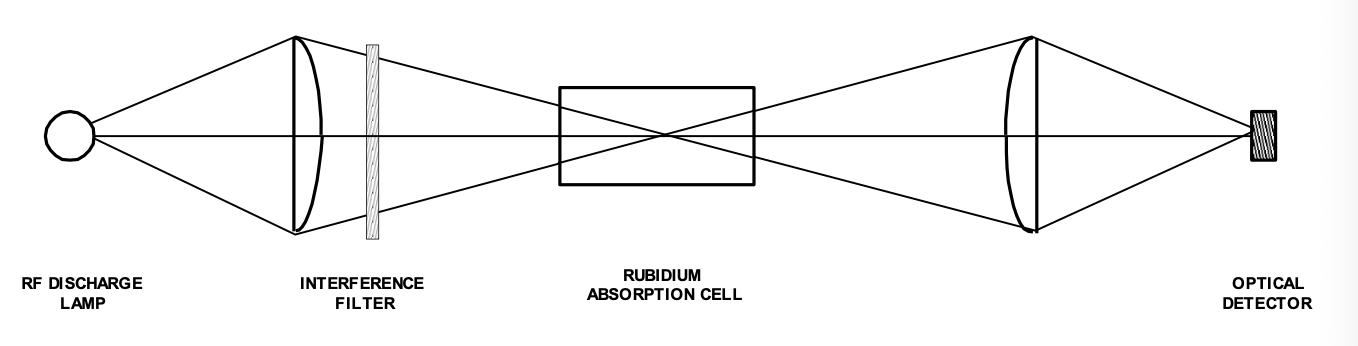
\includegraphics[width=0.5\linewidth]{figures/4a set up.png}
    \caption{Apparatus set up of Experiment A}
    \label{fig:placeholder}
\end{figure}

\subsection{Full Optical Pumping Setup (For Subsequent Experiments)}
For the low field resonance, quadratic Zeeman effect, and transient effect experiments, the setup requires circularly polarized light to achieve a population inversion between the magnetic sublevels.A linear polarizer and a quarter-wave ($\lambda/4$) plate are added between the first lens and the Rb cell. This combination converts the unpolarized lamp light into right or left circularly polarized light ($\sigma^+$ or $\sigma^-$), which is essential for the optical pumping process.\\
\begin{figure}[h]
    \centering
    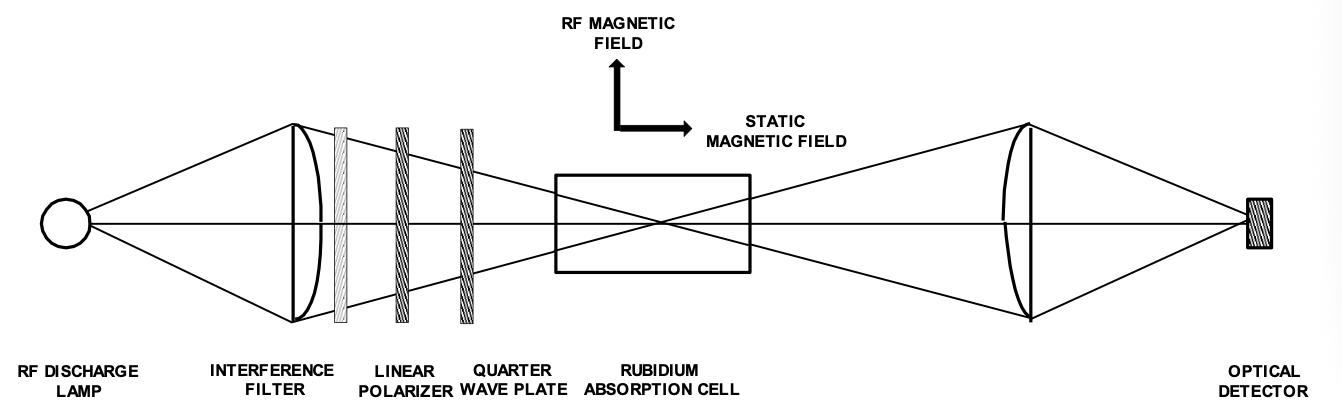
\includegraphics[width=0.5\linewidth]{figures/4b set up.png}
    \caption{Apparatus set up of Experiment B,C and D}
    \label{fig:placeholder}
\end{figure}

\subsection{Magnetic Field Control}The Rb cell is housed within a system of Helmholtz coils.
These coils are used to:
\begin{itemize}
    \item \textbf{Vertical and Horizontal Coils:} Cancel out the Earth’s ambient magnetic field and
    other stray fields to create a "zero-field" environment.
    \item \textbf{Main Coils and Sweep Coils:} Provide a uniform and controllable quantization axis (usually along the optical axis) for observing Zeeman splitting.
    \item \textbf{RF Coils:} A pair of coils perpendicular to the optical axis provides the radio-frequency magnetic field necessary to induce transitions between the magnetic sublevels ($m_F$).
\end{itemize}

\subsection{Electronic System}The photodetector signal is sent to a pre-amplifier and then displayed on an oscilloscope. The RF generator provides the frequency required for resonance, while the sweep generator modulates the magnetic field to allow for the observation of resonance dips on the oscilloscope.

\subsection{Common Measurement Procedure}\label{sec:common_procedure}
All four experiments below share the following operating conventions, stated
here once and not repeated in Sections~\ref{sec:4b}--\ref{sec:4d}. The
photodetector current is amplified by an SRS SR560 pre-amplifier (AC input,
gain 500, LF roll-off \SI{0.1}{\hertz}, HF roll-off \SI{10}{\kilo\hertz}, both
\SI{6}{dB\per octave}) and recorded on a digital oscilloscope. The sweep-coil
and main-coil currents are set on dedicated DC supplies and monitored through
a \SI{0.5}{\ohm} shunt whose voltage reads one-half of the current in amps.
At each set-point the cell thermistor is allowed to stabilise before data
acquisition; the resistive heater is switched off during ODMR measurements to
avoid its stray magnetic field~\cite{OpticalPumpingRubidium2002}. For
spectroscopic runs the oscilloscope is configured in XY mode with the
sweep-coil monitor on CH3 (horizontal reference) and the amplified
photodetector voltage on CH2 (signal); Section~\ref{sec:4d} instead places
the square-wave RF gate on CH1 and records CH2 as a function of time. Each
set-point is repeated across five to six sweep cycles and aggregated with a
combined Type~A/Type~B $u$-value using the meter digitisation
(\SI{0.01}{\volt} or \SI{0.001}{\volt}, as appropriate) as the Type~B floor.
Per-measurement settings (cell-temperature schedule, RF frequency, sweep
rate, drive amplitude) are listed at the top of each subsection below.